\documentclass[12pt]{article}
\usepackage{amssymb,amsmath,amsfonts,bbm,bm,dcolumn,booktabs,eurosym,geometry,ulem,graphicx,color,xcolor,setspace,sectsty,comment,float,caption,pdflscape,subfigure,array,hyperref,listings,tabularx}
\usepackage{xurl}
\usepackage[font=bf]{caption}
\usepackage[bottom]{footmisc}

\lstset{
basicstyle=\small\ttfamily,
columns=flexible,
breaklines=true
}

\hypersetup{
    colorlinks,
    linkcolor={black},
    citecolor={blue!35!black},
    urlcolor={blue!35!black}
}
\normalem
\interfootnotelinepenalty=10000
\setcounter{tocdepth}{2}

\geometry{left=1.0in,right=1.0in,top=1.0in,bottom=1.0in}
\usepackage[style=authoryear,backend=bibtex,maxcitenames=2]{biblatex}
\addbibresource{biblio.bib}

\begin{document}
\title{Exploring Heterogeneous Responses to Text Message Development Programs: An Application of Machine Learning to \textcite{fabregas_digital_2025}}
\author{Steven VanOmmeren\thanks{\href{mailto:sevanommeren@gmail.com}{sevanommeren@gmail.com}. A complete replication package of this project is available at \url{https://github.com/svanomm/development-econ/}.}}
\date{\today}
\maketitle
\noindent
\small
\tableofcontents
\newpage

\doublespacing
\normalsize

\section{Introduction}

The chief concern of development economics is in improving the lives of poor people in the poorest countries of the world. There are many ways to develop an economy; top-down approaches focus on improving the quality of formal and informal institutions in the economy to promote efficient markets, while bottom-up approaches try to equip individuals with the skills and resources they need to improve their lives. A major advancement in the theory of economic development in the 21st century is the use of experiments to guide effective policies.\footnote{See \textcite{basu_influence_2020} for a description of the explosive growth of experiments (and in particular randomized experiments) to measure causal effects of various development policies. An earlier example is \textcite{duflo_use_2003}.} 

In this paper, we study a particular type of bottom-up experiment, grounded in behavioral science, which attempts to steer poor people towards using productivity-increasing technology. Such experiments have historically involved expensive in-person training, but the widespread adoption of mobile phones allows for low-cost text message interventions to be used instead. Text experiments are now being tested in a wide range of contexts, from healthcare to finance to agriculture. We study agricultural experiments in particular, which often center around convincing farmers to adopt new practices or technologies that are expected to improve profitability.

In this paper, we replicate and extend the findings of \textcite{fabregas_digital_2025}, who analyze six randomized controlled trials involving 128,000 farmers in Kenya and Rwanda, finding that text messages modestly but significantly increase the adoption of agricultural lime and fertilizer. The authors are mostly concerned with average treatment effects, but our focus is on the heterogeneity of adoption across different farmer characteristics.

The key hypothesis of this paper is that development policies based in behavioral science would benefit from tailoring the programs to specific groups of people, rather than a one-size-fits-all aproach. In particular, we use the authors' survey data to model lime/fertilizer adoption as a complex, non-linear function of observed characteristics. We show that powerful machine learning models can model the probability of adoption better than the authors' traditional analysis, and then explain how such models could be used for policies going forward. We envision a sophisticated national-scale text program which caters the types of messages sent to each farmer based on their individual characteristics, with the hope of identifying a text program that maximizes the probability of adopting profitable technologies.

The rest of this paper is as follows: the following section reviews the relevant literature on behavioral science, the use of text messages in agricultural development, and our paper of interest. Section \ref{section:methods} describes the data preparation and modeling techniques used in this paper. Section \ref{section:results} presents the results of our models and other analyses. Section \ref{section:discussion} discusses the implications of our findings and their relation to the existing literature. Section \ref{section:conclusion} concludes.

\section{Literature Review}
\label{section:litreview}

\subsection{Behavioral Development Economics}
Results from classical economic theory typically assume that individuals make decisions rationally, with perfect foresight and complete information about the world. But studies in behavioral economics have repeatedly shown that these assumptions do not hold (even approximately) in real life. In particular, many studies in development economics have found that extremely poor people make decisions that may seem irrational or against their own self-interest,\footnote{Of course, irrational decisions are not exclusive to poor people, but a broader discussion of behavioral bias is beyond the scope of this paper.} such as not saving any money, spending excessively on alcohol and tobacco, or failing to adopt productivity-increasing technology. Experimental research in the past 20 years has shown that understanding and correcting these choices can result in increased income at the micro level, leading to economic development at the macro level.

In \textcite{banerjee_understanding_2006} Chapter 24, Esther Duflo explores potential explanations for why Kenyan farmers consistently fail to use fertilizer on their crops, despite it being cheap and profitable. Duflo explains that traditional or ``neoclassical'' explanations such as lack of access to efficient credit markets do not explain the observed behavior. While experimental evidence is inconclusive, Duflo suggests several likely psychological factors at play. For the extremely poor, a bad crop harvest could mean starvation, and so farmers may be extremely risk averse when it comes to adopting new technology.\footnote{Even if the costs involved in experimenting with new fertilizer are low, the small perceived possibility of a bad harvest could be detrimental to the farmer. Additionally, poor farmers may worry that taking on debt to finance investments could lead them to lose their land.} There is also a mental cost associated with learning the new fertilizer techniques that the farmers may overestimate. Duflo found that offering farmers the ability to pay for fertilizer using future crop harvest (instead of cash savings) was able to increase adoption rates. The takeaway of her discussion is that even the neoclassical economic models of the late 20th century are insufficient in explaining the choices of poor people, and that behavioral-inspired interventions should motivate future development policy. 

Behavioral economics has a rich literature focused on identifying the psychological factors involved in everyday economic decision-making. Two important concepts that we review here are ``salience'' and ``nudges.'' These concepts help us understand the basis for text message interventions in development economics, which we discuss later.

In exploring the many heuristics that people use in making decisions, \textcite{tversky_judgment_1974} identify that availability, or the relative ease with which information can be recalled, can bias a person away from rational decisions. Within the topic of availability, ``salience'' describes how ``top-of-mind'' a piece of information is. People process an enormous amount of information each day, and then they forget much of it. Events that occur more recently, or are more emotionally charged, are generally easier to remember. While this is not a particularly surprising idea, salience could explain why people make seemingly irrational decisions. Considering that extremely poor farmers often live in dangerous and dire conditions, they may put knowledge of fertilizer and other technology aside to focus on more immediate concerns. The flip side of this is that salience is an easy bias to influence: simple reminders will make a topic more salient, and thus more likely to be considered in decision-making. This is the basis for many behavioral interventions, including text messages.

\textcite{thaler_nudge_2009}'s concept of ``nudges'' are based on the observation that in some situations, making seemingly small and inexpensive changes to the choices available to people can significantly change their decisions. A classic example of a behavioral nudge is changing the default 401(k) retirement contribution for employees from 0 to some small amount. When the default contribution is 0, employees often do not change it, but when the default is non-zero, they tend to keep the contribution at that level. Employees can still choose to opt out of contributions, but they tend not to, which results in better outcomes for the employees.

\textcite{halpern_nudging_2016} review several examples of successful nudges in policy settings. For example, in the United Kingdom, adding the line ``most people pay their tax on time'' in letters to taxpayers was enough to substantially reduce the amount of late tax filings. Incorporating simple commitment devices like asking job seekers when they will be looking for jobs next week reduced the person-days on welfare by 5 to 10 million, saving the U.K. government as much as \$150 million per year. In summary, the authors highlight that appropriately-designed policy changes based on nudges can bring significant benefits to an economy, provided that they are grounded in good science and are evaluated carefully.

\subsection{Text Experiments}
One promising avenue of nudge policies in development economics is the use of text messages to influence behavior.\footnote{While nudge theory and salience explain part of the reason why text message experiments could improve farmer decisions, there is an information-sharing effect as well. Some farmers simply do not know about recommended technologies, so the texts reveal new information to them. Even still, farmers who did not know about recommended technologies before the experiment may still forget the information and require regular updates to keep the content salient.} Cellphone adoption has increased dramatically in the past 20 years, even in the world's poorest communities. Text messages have very low marginal cost, making them an easy program to justify for a developing economy, and a highly scalable one. In particular, text messages remove the need for in-person visits, which require trained staff and are difficult to scale. Finally, large-scale text message campaigns can be easily randomized, allowing for experimentation, causal inference, and fast iterative improvements. Below, we review the rather mixed results of the literature on text message campaigns in agricultural development economics.

\textcite{fafchamps_impact_2012} represent the earlier end of the literature on text interventions. The authors perform a randomized control trial (RCT) on 1000 farmers in India, in which farmers were offered a subscription to Reuters Market Light, an agricultural information service. The authors estimate an instrumental variables (IV) regression to control for endogenous selection into the subscription service,\footnote{While the experiment randomly assigned the offer of a subscription, not all farmers chose to subscribe. This was a serious issue, as only 59\% of farmers accepted the offer. Further, some farmers subscribed to the program even without the free offer, though this was a much less pervasive issue.} finding little to no benefit from the subscription. Prices obtained by the farmers do not increase after receiving the subscription. Additional models of costs, net prices, revenues, and profits all show no significant differences between the treatment and control groups. It is important to note that the subscription was expected to benefit farmers only by providing more accurate pricing information, not in teaching or reminding them of new agricultural techniques that are known to be more profitable. As we will see in \textcite{fabregas_digital_2025}, the latter type of text message campaign is likely to be more successful.

\textcite{aker_promise_2016} attempt to unify research from disparate fields on the adoption of information and communication technologies (ICTs) in the agricultural sector. The authors explain that there is likely significant heterogeneity in the effectiveness of ICTs for development, using gender as an example. Further, experiments based solely on economic theory may miss the sociological and cultural factors that influence the adoption of ICTs: ``issues such as trust, information quality and the role of gender, caste and ethnicity'' all come into play with regards to the acceptance of ICTs. This makes it difficult to identify the effectiveness of ICT campaigns such as text messages without careful experimentation and a multidisciplinary approach. The authors review several text-based studies with mixed results. For example, \textcite{casaburi_harnessing_2019} found a positive effect of text messages on sugar cane production in Kenya, while \textcite{casaburi_management_2016} found no effect when applying the experiment to a different group of farmers.\footnote{Note that despite the paper dates, \textcite{casaburi_harnessing_2019} data were collected prior to the data used in \textcite{casaburi_management_2016}.}

\textcite{carrion-yaguana_promoting_2020} conduct a randomized control trial in the Tungurahua and Bolivar provinces of Ecuador with a sample size of 292 blackberry farmers. Farmers in the treatment group received a series of text messages reminding them of recommended practices to improve their production (such as applying fertilizer at the right time, pruning branches, and disinfecting tools between uses). Importantly, the messages were sent based on the harvest schedule of blackberry production, so that each text would be relevant and timely. In other words, the recommended practices would be \textit{salient} for the farmers at the right time. Another notable aspect is that the farmers had an average of 10 years of relevant experience going into the study, so they already knew the details of blackberry production, though not necessarily about modern agronomic research. The authors then estimate a multivariate Poisson regression to determine whether the text messages increased the expected number of policies adopted by the farmers, controlling for demographic information such as age, education, and gender. They find mixed results: certain types of policies are adopted more frequently by the treatment group, but others have no significant effect. Further, the authors find heterogeneous effects: less-educated farmers are more likely to be affected by the text messages, while well-educated farmers are not affected. Overall, the results are promising that text messages could provide short-term productivity gains to farmers with mobile phones, but there is clearly a need for larger sample sizes to understand the relatively small effects involved.\footnote{Another weakness of the study is that the outcome is just the adoption of recommended practices, not actual production. Collecting data on subsequent production would have been much more expensive and time consuming. Thus, the underlying assumption is that adopting the recommended practices should increase production on average.}

\subsection{\textcite{fabregas_digital_2025}}
\textcite{fabregas_digital_2025} offers an excellent example of the type of rigorous analysis that is necessary to improve the adoption of text campaigns for economic development. The authors analyze data from six large-scale experiments conducted in Kenya and Rwanda from 2015 to 2019, with a combined sample size of 128,000 farmers. These farmers live in areas with acidic soil that benefits from the application of lime (to reduce acidity) and fertilizer (to speed up growth). Both materials are cheap and available, and are very likely to provide a profit to the farmers in these studies,\footnote{The studies were conducted in areas where soil is highly acidic, which is bad for production. Applying lime decreases the acidity in the soil, nearly guaranteeing a higher crop yield. Applying fertilizer is also nearly guaranteed to increase yield.} yet they have low adoption rates.\footnote{The authors found baseline adoption rates of between 6 and 12 percent for agricultural lime, depending on the sample.} Improving the adoption of lime and fertilizer would provide a small but significant boost to low-income farmers, helping to prop up the local economies. The authors study a relatively simple question: can text messages improve the adoption rates of lime and fertilizer?

The outcome of interest in this analysis is a binary variable indicating whether the farmer adopted the recommended practices of applying lime and fertilizer (a value of 1), or did not adopt them (a value of 0). The authors use two statistical frameworks for analyzing how text messages affect the likelihood of adoption: ordinary least squares (OLS) regression and logistic (or logit) regression. While OLS regression assumes that the outcome variable is continuous and unbounded, it is not uncommon for researchers to use OLS regression on binary outcomes, as OLS can be easier to interpret and understand. Conversely, logistic regression is designed for binary outcomes, and so it is likely the more appropriate model for this analysis. Logistic regressions estimate coefficients for each control variable included in the model. In this case, \textcite{fabregas_digital_2025} report their coefficients as odds ratios, which are interpreted as the relative likelihood of adopting lime/fertilizer. Odds ratios are relative values; when interpreting the treatment effect, a value of 1.2 means that the treatment group is 1.2 times (20\% more) likely to adopt the recommended practices than the control group.

The authors conducted a comprehensive evaluation of the six text message studies, analyzing the studies individually as well as combining them with meta-analysis methodology to assess impacts on farmer adoption of recommended practices. Meta-analysis is a powerful way for the authors to combine the sample sizes of each study to gain statistical precision. In their main results, the authors report that farmers who received the text messages (the treatment group) are 19\% more likely to adopt lime, and 27\% more likely to adopt fertilizer, relative to those who did not receive the text messages (the control group). Both results are statistically significant at the 95\% confidence level. However, their results also show that the individual studies exhibit heterogeneity, with some studies finding no statistically significant treatment effects. Combining the lime and fertilizer studies yields an overall treatment effect of 22\%.

After reporting the statistical models, the authors discuss the cost effectiveness of the text message interventions. The marginal cost of sending one text message is reportedly \$0.01 in these regions, but could be lowered to \$0.001 on a larger scale.\footnote{We can reasonably expect that this price will further decrease over time, following the general trend of decreasing texting costs in developed countries.} Putting that into context, sending 5 text messages to 128,000 farmers (the combined sample size) at a rate of \$0.001 per message would cost only \$640. In contrast, in-person training events cost several dollars per person, per event. Training 128,000 farmers using the authors' estimate of \$9 per person would cost \$1,152,000, or 1,800 times as expensive as a text message program. The authors estimate that the benefit-cost ratio of a large-scale text message program could be as much as 18:1, i.e. \$18 produced for every \$1 spent. Once a text message campaign program is established, the difference between messaging 5,000 farmers and 500,000 farmers is very minimal compared to in-person campaigns.

The analysis of \textcite{fabregas_digital_2025} addresses many of the weaknesses in earlier studies mentioned above. For example, \textcite{fafchamps_impact_2012} used a sample size of 1000 farmers, which is likely insufficient to detect the heterogeneous and relatively small effect sizes of text message programs. \textcite{fabregas_digital_2025} instead combine the results of six studies to get a sample that is orders of magnitude larger. \textcite{casaburi_harnessing_2019} and \textcite{casaburi_management_2016} found conflicting results when studying separate samples; this may not necessarily be a weakness, but \textcite{fabregas_digital_2025} address the problem of multiple samples by studying six different samples that vary over time and geography. Finally, while \textcite{carrion-yaguana_promoting_2020} measure the adoption of recommended practices by a self-reported survey, \textcite{fabregas_digital_2025} address the potential for bias by studying administrative data that confirms whether farmers actually purchased the recommended inputs, rather than simply saying they did.\footnote{In either case, the authors do not analyze resulting farmer production, which would be the ideal outcome to assess profitability of the text campaigns.}

While the purpose of the \textcite{fabregas_digital_2025} analysis was to determine aggregate effectiveness of text messages for large-scale policy recommendations, the authors also perform a few sensitivity analyses to explore potential heterogeneous responses to the text messages. The authors run separate regressions for different subpopulations of their data, such as females only, people with primary education only, and young people only. While there are some differences in the treatment effect measured by each regression, they ``find no evidence of a statistically significant differential program effect by these characteristics,'' even when pooling the studies to increase sample size. 

However, there are a few weaknesses of the authors' heterogeneity analysis. First, the authors only study heterogeneous effects separately for each demographic variable; they do not attempt to interact the controls with each other. Second, the authors only tested logistic and OLS regressions. It is possible that the relationship between observed demographics and treatment effects are more complex than these basic models can capture. Based on the discussion in \textcite{aker_promise_2016}, it is surprising for \textcite{fabregas_digital_2025} to find no indication of heterogeneous effects. The purpose of our analysis is to further explore the authors' data to see if heterogeneity exists in a more nuanced way than the authors investigated.

\section{Methods}
\label{section:methods}

\subsection{Data Preparation}
\textcite{fabregas_digital_2025} graciously provide a detailed Online Appendix and replication package for their results, which includes the data used in their regression analyses.\footnote{\url{https://www.openicpsr.org/openicpsr/project/186241/version/V1/view}.} We began by running all of their Stata code to build their regression datasets, as well as replicating their regression results.

We sourced additional data from the World Bank Group. The World Development Indicators (WDI) database provides a variety of country-level statistics by country and year.\footnote{\url{https://datacatalog.worldbank.org/search/dataset/0037712}.} We selected the following variables for our analysis:
\begin{itemize}
    \singlespacing
    \item Mobile cellular subscriptions (per 100 people)
    \item Individuals using the Internet (\% of population)
    \item GNI per capita, PPP (constant 2021 international \$)
    \item Literacy rate, adult total (\% of people ages 15 and above)
\end{itemize}
After filtering the data to these variables, we selected the following countries: Kenya, Rwanda, Ecuador, India, and United States. This list includes the countries mentioned in the text experiments discussed above, as well as the United States as a reference developed country. We selected data from 2010 to 2023 to analyze trends over time; this period includes the time during which the \textcite{fabregas_digital_2025} experiments were conducted.

\subsection{Modeling}
We study the models underlying Table E2 in the \textcite{fabregas_digital_2025} Online Appendix. This table reports the results of 24 regressions: 6 logit and 6 OLS models, each of which is run on both the lime and the fertilizer recommendations. These are ``pooled'' models that combine the data from all the experiments that include the relevant controls. Because OLS is not ideal for studying binary outcomes, we only report the logit models. Each model uses the following specification:\footnote{Each model also includes fixed effects for each of the six experiments as well as interactions between the demographic variable and the program fixed effects. We do not report these terms in the equation to be consistent with the original paper.}
\begin{equation}
    \mathbbm{1}[\text{Followed Recommendations}_i] = \alpha \cdot \text{Treated}_i + \beta \cdot X_i + \gamma \cdot (\text{Treated}_i \times X_i) + \epsilon_i,
\end{equation}
where Treated is an indicator for whether farmer $i$ was in the treatment group (received texts), $X$ is a demographic variable of interest, and $(\text{Treated}_i \times X_i)$ measures the interaction between the treatment and the demographic variable. $\epsilon$ is the error term. The following 6 variables are used for $X$:\footnote{To clarify, the model does not include all 6 variables simultaneously. $X$ denotes a single variable, and so 6 separate regressions are run, substituting $X$ for one of the variables discussed here.}
\begin{itemize}
    \singlespacing
    \item Female
    \item Primary: whether respondent completed primary school
    \item Large Farm: more than 1.5 acres of land
    \item Young: under 40 years old
    \item Used Input: whether the respondent had previously used lime/fertilizer
    \item Heard Input: whether the respondent had previous knowledge of lime/fertilizer or was aware of it
\end{itemize}

The authors report only the regression coefficients, the sample size, and the mean outcome for the control group. They do not report any measures of model fit. We modify their code to report two measures of classification accuracy: the balanced accuracy statistic and the area under the receiver operating characteristic curve (AUROC). The balanced accuracy statistic is defined as the average of the true positive rate and true negative rate,\footnote{Balanced accuracy depends on the model's classification threshold. For each model, we determined the threshold that maximizes balanced accuracy. For the logit models, this was determined by simply testing all possible probabilities calculated by the model (there were only a handful of unique values), while for the LightGBM models we use an optimization algorithm from the Python package \textsf{scikit-learn}.} and is a good measure of model fit for binary outcomes on imbalanced data.\footnote{This dataset is highly imbalanced in the outcomes, as only a small portion of the farmers ended up purchasing lime or fertilizer.} The AUROC is a measure of how well the model can distinguish between the two classes at various classification thresholds and so provides an overall summary of its usefulness. Both measures range from 0 to 1, with a higher value indicating a better model. A value of 0 means that the model always predicts the wrong value. A value of 0.5 indicates that the model is as good as random guessing. A value of 1 means that the model perfectly predicts the outcome.

An additional important note is that not all demographics were collected in each experiment, so the sample size differs among the models. This is likely why the authors did not try to combine demographics into a single model.

Next, we implement a machine learning technique called LightGBM. LightGBM is a histogram-based gradient boosting tree model from \textcite{ke_lightgbm_2017}, created as an extension to the popular XGBoost (extreme gradient boost) technique. The model works by iteratively splitting the data into ``branches'' of if-then statements that best fit the outcome variable. By repeatedly fitting new trees onto the residuals of existing trees, the model learns complex relationships that can approximate any function. LightGBM is widely known as a versatile machine learning technique that works remarkably well with large tabular data. An important aspect of LightGBM for our purposes is that it natively supports missing values by treating them as a distinct value in the splitting procedure. This is useful because the model can include all 128,000 observations from the data, whereas a logit model would remove any rows of data with a missing variable.

We test a total of six LightGBM models. There are two feature sets of interest: a `basic' set of features that correspond to the same controls used by \textcite{fabregas_digital_2025}, and a `large' model that includes additional controls from the data and interaction terms.\footnote{Specifically, we include the following features: treatment indicator, female indicator, primary school indicator, ever used lime indicator, ever heard of lime indicator, program fixed effects, family-oriented text message, farm size, farm size squared, age (in decades), age squared, number of messages sent, number of messages sent squared, estimated farm acidity (calculated as 7 minus the estimated pH of the farm soil), estimated farm acidity squared. We interact each variable except the program fixed effects with the treatment indicator. We interact the female indicator with the remaining controls, and also interact the ever used lime indicator with the remaining controls. There are 52 variables in total.} These two feature sets are run on three subsets of the data: a model predicting the adoption of lime, a model for fertilizer, and a model that predicts both lime and fertilizer adoption. All LightGBM models use the following hyperparameters: learning rate of 0.01, sample weights to balance the outcome classes, minimum samples per leaf of 31, $L2$ regularization of 0, maximum features of 1.0, no maximum tree depth, maximum iterations of 2000, and early stopping if the AUROC does not improve after 100 training iterations. We did not perform a formal hyperparameter tuning analysis, but found via experimentation that hyperparameter changes did not appear to significantly impact model performance. All models were trained and evaluated using the \textsf{scikit-learn} package developed by \textcite{pedregosa_scikit-learn_2018}.

\section{Results and Analysis}
\label{section:results}
\subsection{Summary Analysis}
Below, we plot the national average of mobile cellular subscriptions per 100 people using the World Bank Group data. Figure \ref{fig:mobile_subscriptions} shows that the average number of mobile subscriptions has increased dramatically in Kenya and Rwanda since 2010, while the United States has remained relatively constant. According to the data, Ecuador saw a decrease in mobile subscriptions from 2014 to 2015, with a slow recovery since then. India's increase in subscriptions has been relatively slow, on par with the United States. 

While in 2010, Rwanda had fewer than 40 subscriptions per 100 people (less than half of the United States), it had about 75 subscriptions per 100 people by 2019 (the last year of data collection in \textcite{fabregas_digital_2025}). Rwanda saw relatively little growth during the 2015 to 2019 period.

Kenya had about 60 subscriptions per 100 people in 2010, nearly twice as many as in Rwanda. By 2015, the country had 80 subscriptions and, unlike Rwanda, saw a striking amount of growth in mobile subscriptions from 2015 to 2019, with the country reportedly surpassing the United States by 2019. As of 2023, the country reportedly had 120 subscriptions per 100 people, compared to about 110 in the United States. Overall, Figure \ref{fig:mobile_subscriptions} shows that mobile phone ownership has considerably increased in the developing countries involved in our studies, suggesting that text-based development programs can effectively reach a large proportion of the population.\footnote{Note that this chart does not show what percent of the population owns a mobile phone. People can have multiple subscriptions, and this chart does not explain the distribution of phone ownership in the population. Phone ownership is likely unequally distributed, with poor people being less likely to own a phone than rich people within the country.}
\begin{figure}[H]
    \centering
    \caption{National Average of Mobile Cellular Subscriptions per 100 People}
    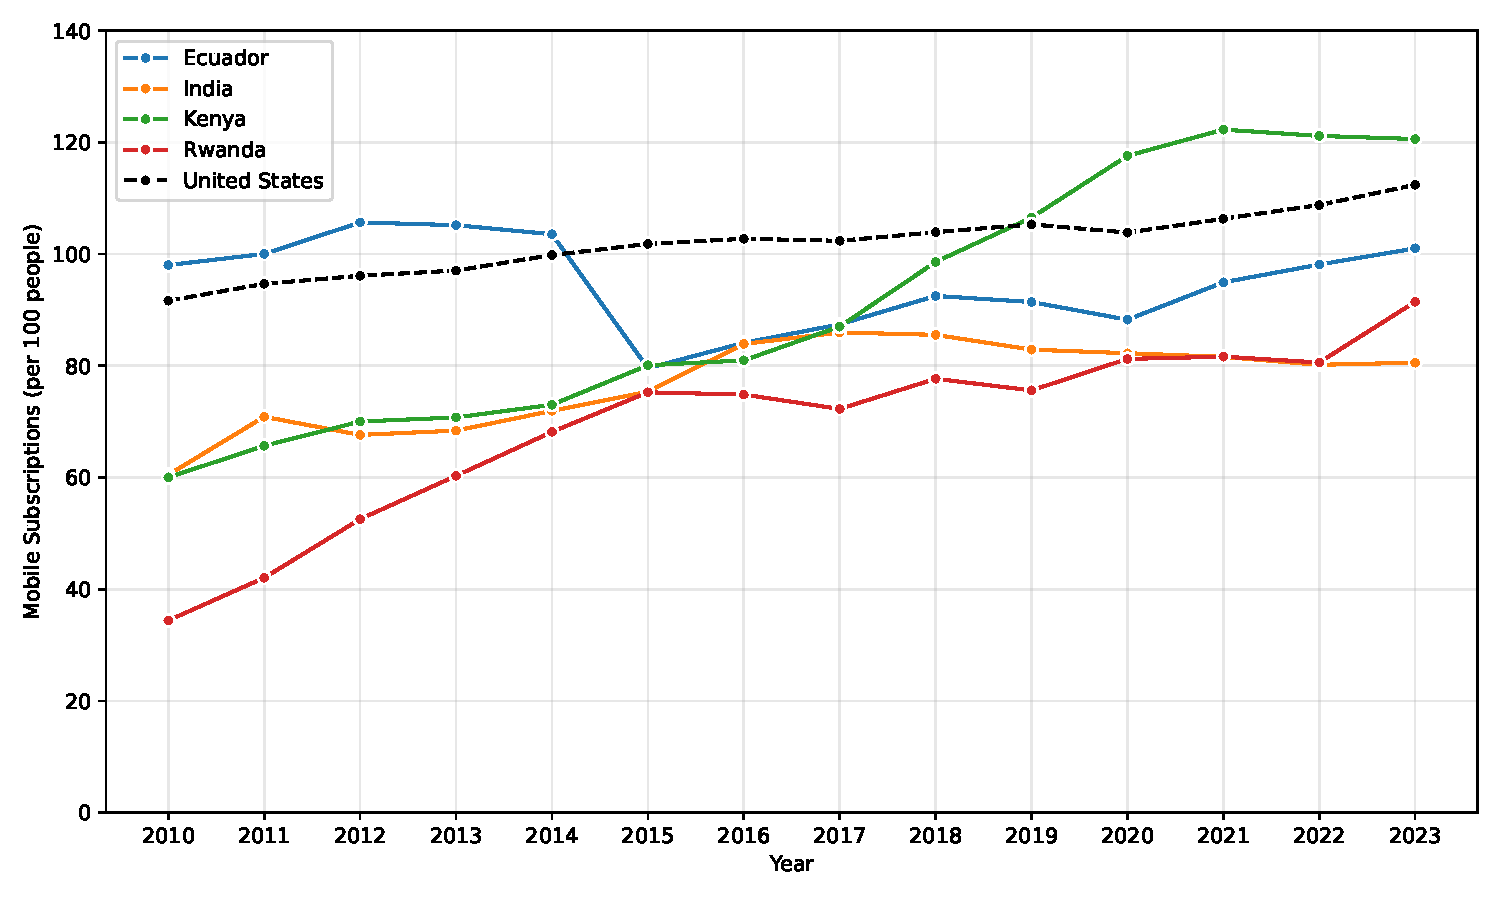
\includegraphics[width=\textwidth]{../output/mobile_subscriptions.pdf}
    \begin{minipage}{0.9\textwidth}
    \footnotesize
    Source: World Bank Group, World Development Indicators (WDI) database. 
    \end{minipage}
    \label{fig:mobile_subscriptions}
\end{figure}

Next, we report the percent of individuals using the Internet by country and year. Figure \ref{fig:internet_use} shows that while Internet usage has substantially increased in all countries, it is still relatively low in Kenya and Rwanda. As of 2023, both countries were at around 35\% of the population, as opposed to over 70\% in Ecuador and over 90\% in the United States.\footnote{Internet usage for India was not available in 2023 in our dataset.} During the 2015-2019 period of the \textcite{fabregas_digital_2025} studies, fewer than 1 in 5 people used the Internet in Kenya and Rwanda.

Comparing Figure \ref{fig:internet_use} with Figure \ref{fig:mobile_subscriptions} shows that text message-based experiments are a better policy to pursue compared to social media-based interventions for Kenya and Rwanda (given their relatively low Internet usage). But for other countries like Ecuador, Internet use is high enough that social media could be a viable tool for nudge experiments.

\begin{figure}[H]
    \centering
    \caption{Percent of Individuals using the Internet}
    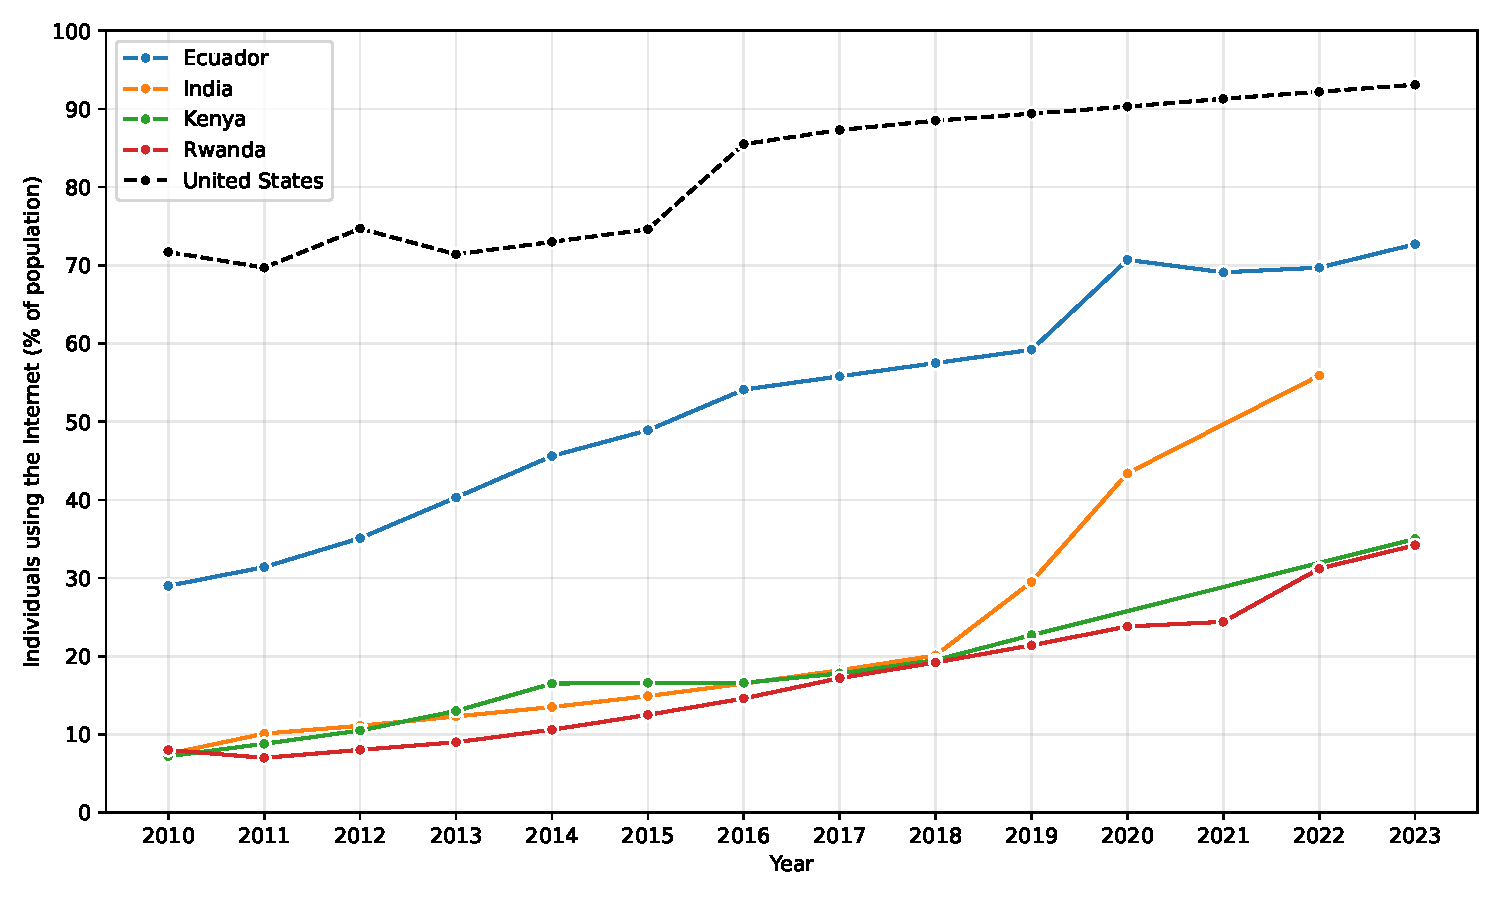
\includegraphics[width=\textwidth]{../output/individuals_using_internet.pdf}
    \begin{minipage}{0.9\textwidth}
    \footnotesize
    Source: World Bank Group, World Development Indicators (WDI) database. 
    \end{minipage}
    \label{fig:internet_use}
\end{figure}

Finally, we report the national literacy rates for each country. Unfortunately, literacy data was missing for several years in our database for the given countries. Regardless, connecting the available data points shows that literacy rates have slowly increased over time for each country. In 2010, Rwanda had a literacy rate of about 66\%, which increased to 79\% by 2022. Ecuador has the highest literacy rate in this chart, increasing from 92\% to 94\% from 2010 to 2022.\footnote{United States literacy rate was not available in this data. Using a comparable definition of basic literacy (as opposed to more advanced reading/writing ability), the U.S. would likely have a literacy rate of approximately 100\%. \url{https://worldpopulationreview.com/country-rankings/literacy-rate-by-country}.} This chart shows that literacy rate is likely the bottleneck in introducing text message interventions in developing countries, with literacy being lower than phone ownership in Kenya and Rwanda.\footnote{Note that text message interventions need not necessarily require literacy. A carefully crafted series of emojis, pictures, and videos could convey helpful information without requiring text comprehension.}

\begin{figure}[H]
    \centering
    \caption{National Adult Literacy Rates}
    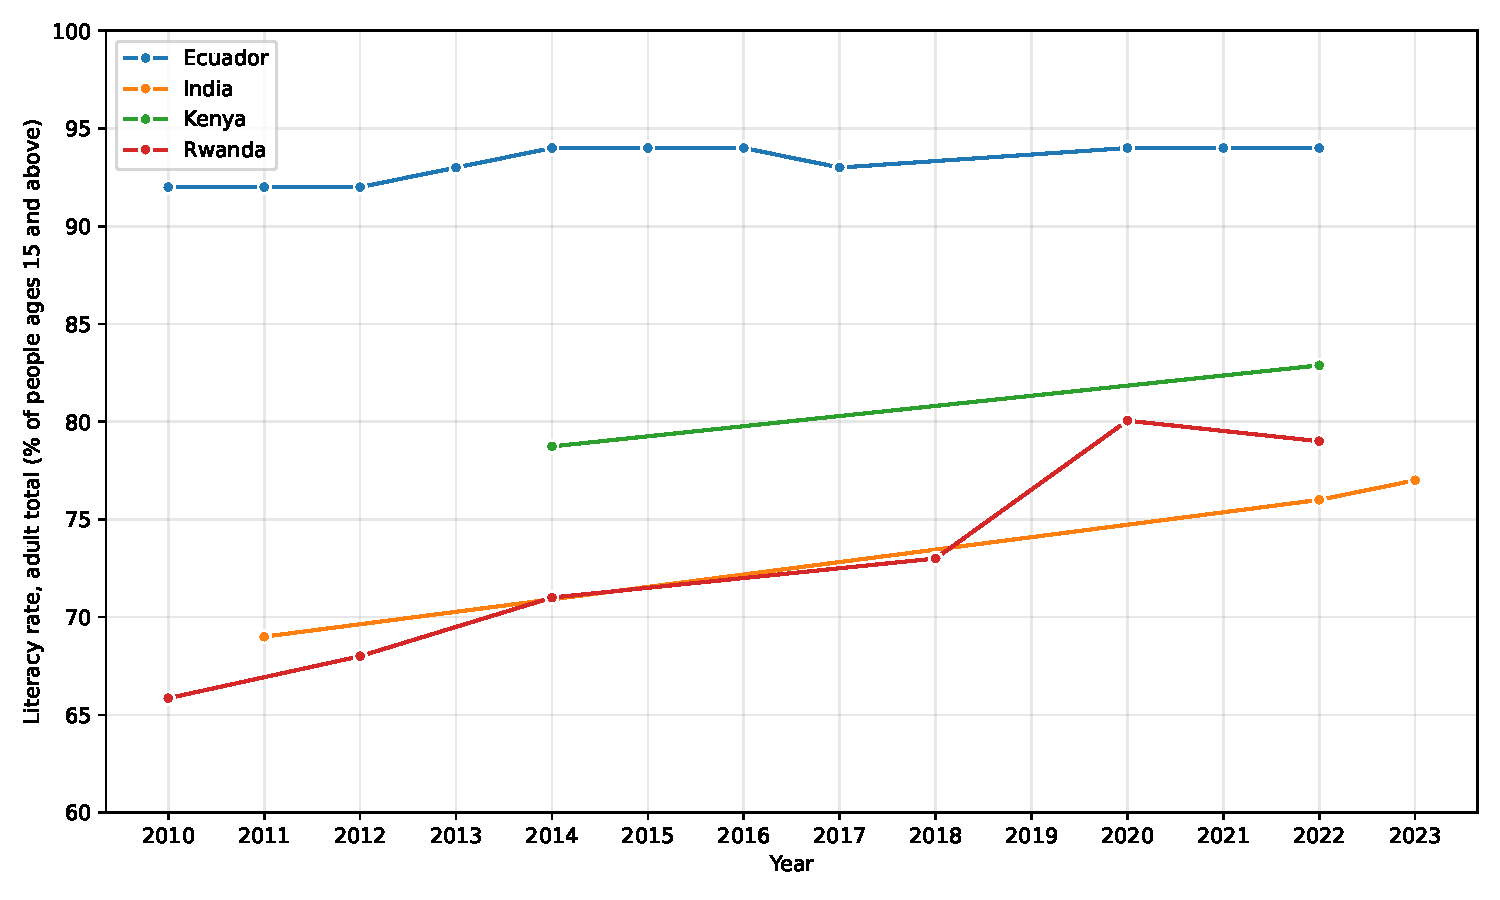
\includegraphics[width=\textwidth]{../output/literacy_rate.pdf}
    \begin{minipage}{0.9\textwidth}
    \footnotesize
    Source: World Bank Group, World Development Indicators (WDI) database. 
    \end{minipage}
    \label{fig:literacy_rate}
\end{figure}

\subsection{Model Fit}
Below, we report our replication of the heterogeneity regressions from \textcite{fabregas_digital_2025}, where we have added model fit statistics for each model.

\begin{table}[H] \centering
\newcolumntype{R}{>{\raggedleft\arraybackslash}X}
\newcolumntype{L}{>{\raggedright\arraybackslash}X}
\newcolumntype{C}{>{\centering\arraybackslash}X}

\caption{Replicated Heterogeneity Logit Models: Lime}
\resizebox{0.8\columnwidth}{!}{
\begin{tabularx}{\linewidth}{@{}lCCCCCC@{}}

\toprule
{Variable}&{Female}&{Primary}&{Large Farm}&{Young}&{Used Input}&{Heard Input} \tabularnewline
\midrule \addlinespace[\belowrulesep]
Treated&1.183$^{***}$&1.115&1.146$^{***}$&1.101$^{***}$&1.162$^{***}$&1.078 \tabularnewline
&(0.054)&(0.113)&(0.032)&(0.034)&(0.042)&(0.073) \tabularnewline
$[X]$&0.729&1.979$^{**}$&1.204&1.066&0.520&0.715 \tabularnewline
&(0.173)&(0.542)&(0.342)&(0.257)&(0.291)&(0.204) \tabularnewline
$[X]$ *Treated&0.938&1.055&0.994&1.055&1.020&1.245$^{*}$ \tabularnewline
&(0.048)&(0.132)&(0.042)&(0.047)&(0.101)&(0.145) \tabularnewline
\midrule Program FE&Yes&Yes&Yes&Yes&Yes&Yes \tabularnewline
Mean Control&0.29&0.23&0.13&0.31&0.06&0.25 \tabularnewline
AUROC&0.59&0.60&0.79&0.56&0.72&0.58 \tabularnewline
Best Threshold&0.31&0.25&0.14&0.33&0.06&0.28 \tabularnewline
Balanced Accuracy&0.57&0.58&0.76&0.55&0.71&0.56 \tabularnewline
Observations&44,969&9,711&128,889&40,164&91,433&8,560 \tabularnewline
\bottomrule \addlinespace[\belowrulesep]
\end{tabularx}
}
\\ \parbox{0.79\linewidth}{\tiny Pooled models combine the data from all studies with sufficient data. The dependent variable is whether the farmer followed recommendations for lime or fertilizer. 'Program FE' are fixed effects for each available study; we also include interactions with the control variable. Coefficients are reported as odds ratios. 'AUROC' is the area under the receiver operator curve (higher is better). 'Best Threshold' is the classification threshold that maximizes balanced accuracy. 'Balanced Accuracy' is the average of classification sensitivity and specificity (higher is better).}
\end{table}

\begin{table}[H] \centering
\newcolumntype{R}{>{\raggedleft\arraybackslash}X}
\newcolumntype{L}{>{\raggedright\arraybackslash}X}
\newcolumntype{C}{>{\centering\arraybackslash}X}

\caption{Replicated Heterogeneity Logit Models: Fertilizer}
\resizebox{0.8\columnwidth}{!}{
\begin{tabularx}{\linewidth}{@{}lCCCCCC@{}}
\toprule
{Variable}&{Female}&{Primary}&{Large Farm}&{Young}&{Used Input}&{Heard Input} \tabularnewline
\midrule \addlinespace[\belowrulesep]
Treated&1.105$^{*}$&1.228&1.104$^{**}$&1.095$^{**}$&1.124$^{**}$&1.432 \tabularnewline
&(0.065)&(0.239)&(0.055)&(0.044)&(0.054)&(0.619) \tabularnewline
$[X]$&1.157&1.491$^{**}$&0.737$^{**}$&1.044&0.973&1.054 \tabularnewline
&(0.170)&(0.275)&(0.100)&(0.149)&(0.158)&(0.404) \tabularnewline
$[X]$ *Treated&1.013&0.935&1.041&1.062&1.062&0.751 \tabularnewline
&(0.069)&(0.220)&(0.083)&(0.086)&(0.095)&(0.363) \tabularnewline
\midrule Program FE&Yes&Yes&Yes&Yes&Yes&Yes \tabularnewline
Mean Control&0.13&0.08&0.13&0.13&0.13&0.41 \tabularnewline
AUROC&0.63&0.80&0.61&0.63&0.76&0.52 \tabularnewline
Best Threshold&0.13&0.03&0.03&0.14&0.09&0.41 \tabularnewline
Balanced Accuracy&0.59&0.78&0.59&0.59&0.72&0.51 \tabularnewline
Observations&40,157&8,560&41,132&40,164&41,132&773 \tabularnewline
\bottomrule \addlinespace[\belowrulesep]
\end{tabularx}
}
\\ \parbox{0.79\linewidth}{\tiny Pooled models combine the data from all studies with sufficient data. The dependent variable is whether the farmer followed recommendations for lime or fertilizer. 'Program FE' are fixed effects for each available study; we also include interactions with the control variable. Coefficients are reported as odds ratios. 'AUROC' is the area under the receiver operator curve (higher is better). 'Best Threshold' is the classification threshold that maximizes balanced accuracy. 'Balanced Accuracy' is the average of classification sensitivity and specificity (higher is better).}
\end{table}


Viewing the replicated results from \textcite{fabregas_digital_2025}, we find that the AUROC, best threshold, and balanced accuracy vary substantially between models. For predicting lime, the model that includes all observations (Large Farm) has an AUROC of 0.79 and balanced accuracy of 0.76.\footnote{This model fit is due almost entirely to the program fixed effects. Removing the treatment variable, control, and interaction terms yields an AUROC of 0.78, which is only slightly worse.} The other controls are missing for many observations, and for the lime prediction this results in worse AUROC. But this does not hold for fertilizer, where the models with the most number of observations (Large Farm and Used Input) have AUROCs that are worse than a model with less than a quarter of the observations (Primary).

One takeaway from the replicated results is that model performance seems to be incomparable when the observation count differs. The value of Mean Control (i.e. adoption rates for the control group) is so different across models that it complicates direct comparisons.

While it would have been helpful to include all the controls mentioned in the tables above in a single logit model to assess overall heterogeneity, this is unfortunately not possible. Because of differing data collection between the experiments, there are no records that have non-missing values for all of the controls, so a standard logit model will not run on the data.\footnote{We did not experiment with data imputation techniques, which could have helped alleviate this issue. However, we do not believe that data imputation would solve all issues. For example, the `heard input' variable is only available for 773 fertilizer observations. It would be almost completely uninformative to impute this on the remaining 40,000 observations in the data.} Thus, to compare against the LightGBM models, we use the best-performing model that includes all observations from the tables above, i.e. the `Large Farm' lime model and `Used Input' fertilizer model.

We now report the best logit models from \textcite{fabregas_digital_2025} against two LightGBM specifications: a basic model which includes all control variables from the tables above, and a larger model which includes additional variables and interaction terms not used by the authors. Recall that because LightGBM models natively support missing values, they can include all observations in the data while still using all the control variables.

\begin{table}[H] \centering
\newcolumntype{R}{>{\raggedleft\arraybackslash}X}
\newcolumntype{L}{>{\raggedright\arraybackslash}X}
\newcolumntype{C}{>{\centering\arraybackslash}X}

\caption{Model Results Comparison: Lime}
\resizebox{0.8\columnwidth}{!}{
\begin{tabularx}{\linewidth}{@{}lCCC@{}}
\toprule
{Statistic}&{\footnotesize Original (Large Farm)}&{Basic Model}&{Large Model} \tabularnewline
\midrule AUROC&0.79&0.81&0.84 \tabularnewline
Best Threshold&0.14&0.51&0.57 \tabularnewline
Balanced Accuracy&0.76&0.77&0.78 \tabularnewline
Observations&128,889&128,889&128,889 \tabularnewline
\bottomrule \addlinespace[\belowrulesep]
\end{tabularx}
}
\\ \parbox{0.79\linewidth}{\tiny The dependent variable is whether the farmer followed recommendations for lime or fertilizer. 'Original (Large Farm)' is a heterogeneity model from \textcite{fabregas_digital_2025}. 'Basic Model' is a LightGBM classification model that includes the variables tested by \textcite{fabregas_digital_2025}. 'Large Model'  is a LightGBM classification model that includes additional variables and interactions. 'AUROC' is the area under the receiver operator curve (higher is better). 'Best Threshold' is the classification threshold that maximizes balanced accuracy. 'Balanced Accuracy' is the average of classification sensitivity and specificity (higher is better).}
\end{table}

\begin{table}[H] \centering
\newcolumntype{R}{>{\raggedleft\arraybackslash}X}
\newcolumntype{L}{>{\raggedright\arraybackslash}X}
\newcolumntype{C}{>{\centering\arraybackslash}X}

\caption{Model Results Comparison: Fertilizer}
\resizebox{0.8\columnwidth}{!}{
\begin{tabularx}{\linewidth}{@{}lCCC@{}}
\toprule
{Statistic}&{\footnotesize Original (Used Input)}&{Basic Model}&{Large Model} \tabularnewline
\midrule AUROC&0.76&0.65&0.86 \tabularnewline
Best Threshold&0.09&0.49&0.46 \tabularnewline
Balanced Accuracy&0.72&0.61&0.78 \tabularnewline
Observations&41,132&41,132&41,132 \tabularnewline
\bottomrule \addlinespace[\belowrulesep]
\end{tabularx}
}
\\ \parbox{0.79\linewidth}{\tiny The dependent variable is whether the farmer followed recommendations for lime or fertilizer. 'Original (Large Farm)' is a heterogeneity model from \textcite{fabregas_digital_2025}. 'Basic Model' is a LightGBM classification model that includes the variables tested by \textcite{fabregas_digital_2025}. 'Large Model'  is a LightGBM classification model that includes additional variables and interactions. 'AUROC' is the area under the receiver operating curve (higher is better). 'Best Threshold' is the classification threshold that maximizes balanced accuracy. 'Balanced Accuracy' is the average of classification sensitivity and specificity (higher is better).}
\end{table}


Viewing the results in the tables above, we see that the large LightGBM model outperforms the logit and basic LightGBM model for both lime and fertilizer predictions. For predicting lime, LightGBM models provide a relatively marginal improvement in AUROC and balanced accuracy: the large model has an AUROC of 0.84 vs the logit model's 0.79, and a balanced accuracy of 0.78 vs 0.76. There are larger improvements when predicting fertilizer, with the large model yielding an AUROC of 0.86 vs the logit's 0.76, and a balanced accuracy of 0.78 vs 0.72. While the basic LightGBM model slightly outperforms the logit in predicting lime, it is noticeably worse than the logit in predicting fertilizer usage.

Finally, we tested a LightGBM model which combines lime and fertilizer to see how well a model could predict the overall decision to adopt the suggested agricultural inputs. The basic model has an AUROC of 0.75 and balanced accuracy of 0.71, while the large model has an AUROC of 0.82 and balanced accuracy of 0.76. This suggests that there are likely some common factors governing the choice to adopt agricultural inputs, and that they can be predicted fairly accurately. See the Appendix, Section \ref{sec:combined_model} for more information about this model.

\subsection{Model Predictions}
Machine learning models like LightGBM are often considered ``black boxes'' because they do not provide an interpretable set of coefficients for the control variables. Whereas in the logit model, we can report the odds ratios estimated by the model, we need to be more creative in interpreting the LightGBM models. We assess how important our controls are to the models' performance through the use of Shapley values.\footnote{We calculate Shapley values using a method developed by \textcite{lundberg_unified_2017}, as incorporated in the Python package \textsf{shap}.} Shapley values attribute the importance of each feature for a given model through the mechanics of cooperative game theory.\footnote{We use the terms ``control variables'', ``controls,'' and ``features'' interchangeably here and below.} Shapley values estimate how much the given feature contributes to the model's final prediction. For example, if a feature has a Shapley value of 100, then the model's prediction is 100 higher than it would be without that feature. A higher Shapley value (in absolute value) means that the feature contributes more to the model's predictions, meaning it is more important.

In Figure \ref{fig:shap_force}, we report two examples of how Shapley values can be used to understand the LightGBM large model, predicting lime usage. We sampled 1000 farmers from the data and identified the farmer with the lowest estimated probability of adoption (in orange) and the highest probaility (in blue). The charts are read from top to bottom: both farmers start out with a baseline probability of 40.4\%. We then incorporate the Shapley values for each control variable to see how it changes the predicted probability of using lime, with the bottom bars representing the model's final prediction.\footnote{For the sake of clarity, we have omitted controls with near-zero Shapley values.} For example, the orange farmer's predicted probability increases from a baseline of 40.4\% to 41.3\% when we incorporate the indicator for whether he/she has used lime before (which is missing in this case). 

\begin{figure}[H]
    \centering
    \caption{Shapley Waterfall Plot Examples, Large Model: Lime}
    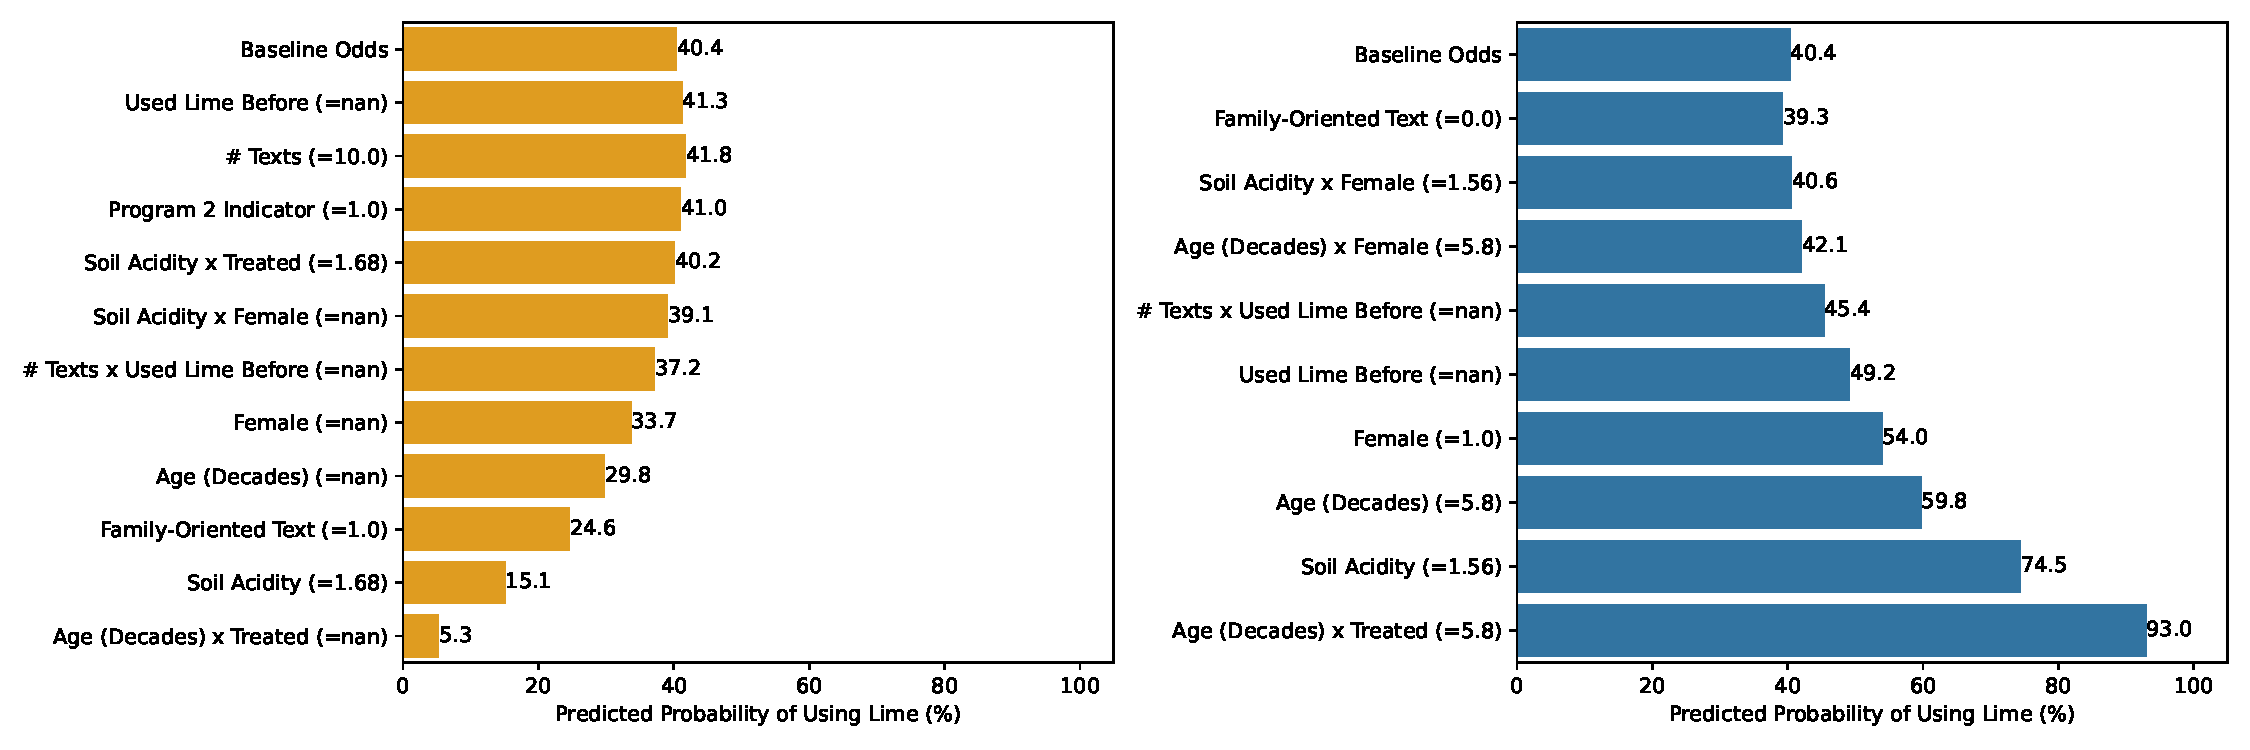
\includegraphics[width=\textwidth]{../output/shap_forceplot_examples_lime.pdf}
    \begin{minipage}{0.8\textwidth}
    \tiny
    Shapley values estimate how much each feature value contributes to the model's estimated probability of following recommendations for lime. We sampled 1000 farmers and selected the smallest and largest estimated probability. The charts show how the model goes from a baseline probability value (at the top) to the final prediction (the bottom) as we incorporate the control variables, step by step. Each bar is a separate control variable, and the values in parentheses are the observed value for the given farmer. Shapley values here are given by the difference between each bar.
    \end{minipage}
    \label{fig:shap_force}
\end{figure}

Comparing the two farmers, one difference that stands out is that the blue farmer is identified as female, while the orange farmer's female status is unknown. The model attributes an increased probability of using lime for the blue farmer because of her female status: +1.3\% because of the interaction of soil acidity and female, +1.5\% because of the interaction between age and female, and +4.8\% from the female indicator alone. The largest positive effect on the predicted probability comes from the variable `Age (Decades) x Treated', which indicates that the model thinks this 58-year-old farmer who received text messages is highly receptive to adopting lime. Conversely, the orange farmer has an unknown age, which decreases the model's predicted probability.

Figure \ref{fig:shap_force} demonstrates that the model finds heterogeneous responses to the text messages. Note that for both farmers, the ``Treated'' variable alone is not included in the charts; this is because the model found that it did not contribute to the predicted probability of adoption. Instead, we see that the interaction of age and treatment was very important for both farmers, suggesting that certain age groups are more receptive to the texts than others.

Shapley values are neither linear nor homogenous across observations, and so we cannot expect that all 58-year-old farmers who received text messages should have an increased probability of adopting lime or fertilizer. Figure \ref{fig:shap_lime} and Figure \ref{fig:shap_fert} show the distribution of Shapley values from the lime/fertilizer models for a sample of 1000 farmers. Each row in the charts reports the distribution for a given feature, where the $x$-axis is the Shapley value (increased/decreased predicted probability of adoption), the colors indicate whether the feature's observed value is low (blue), high (red), or missing (gray) for each farmer, and the height represents the frequency distribution of values.

\begin{figure}[H]
    \centering
    \caption{Top Shapley Value Distributions, Large Model: Lime}
    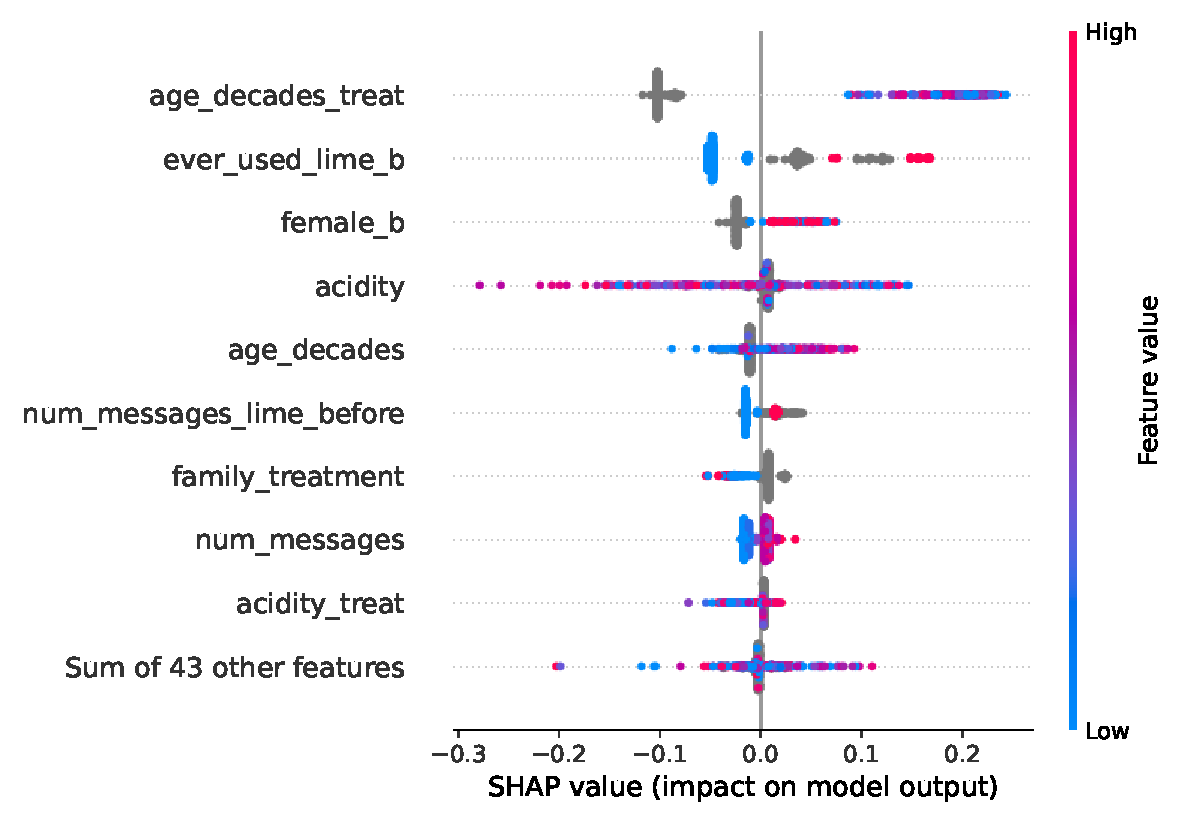
\includegraphics[width=0.7\textwidth]{../output/shap_beeswarm_lime.pdf}
    \begin{minipage}{0.7\textwidth}
    \tiny
    Shapley values estimate how much each feature value contributes to the model's estimated probability of following recommendations for lime/fertilizer. A higher SHAP value (the x-axis) means that the model predicts a higher probability than it would without that feature. Shown here are the top 10 features by average absolute SHAP value. Dots in this graph are blue when the respective feature is a lower value, and red when the respective feature is a higher value. Gray dots indicate missing values for the respective feature.
    \end{minipage}
    \label{fig:shap_lime}
\end{figure}

The distributions of values in Figure \ref{fig:shap_lime} for predicting lime adoption show that missing values clearly affect the predicted probabilities. The first row (a variable for age interacted with treatment status) has negative Shapley values when missing, and positive values for both low or high non-missing values. The second row shows that when the farmer has never used lime before, the model expects the farmer to have a lower adoption rate, while it predicts a higher value for those who have used lime before and a smaller positive effect for missing values.

\begin{figure}[H]
    \centering
    \caption{Top Shapley Value Distributions, Large Model: Fertilizer}
    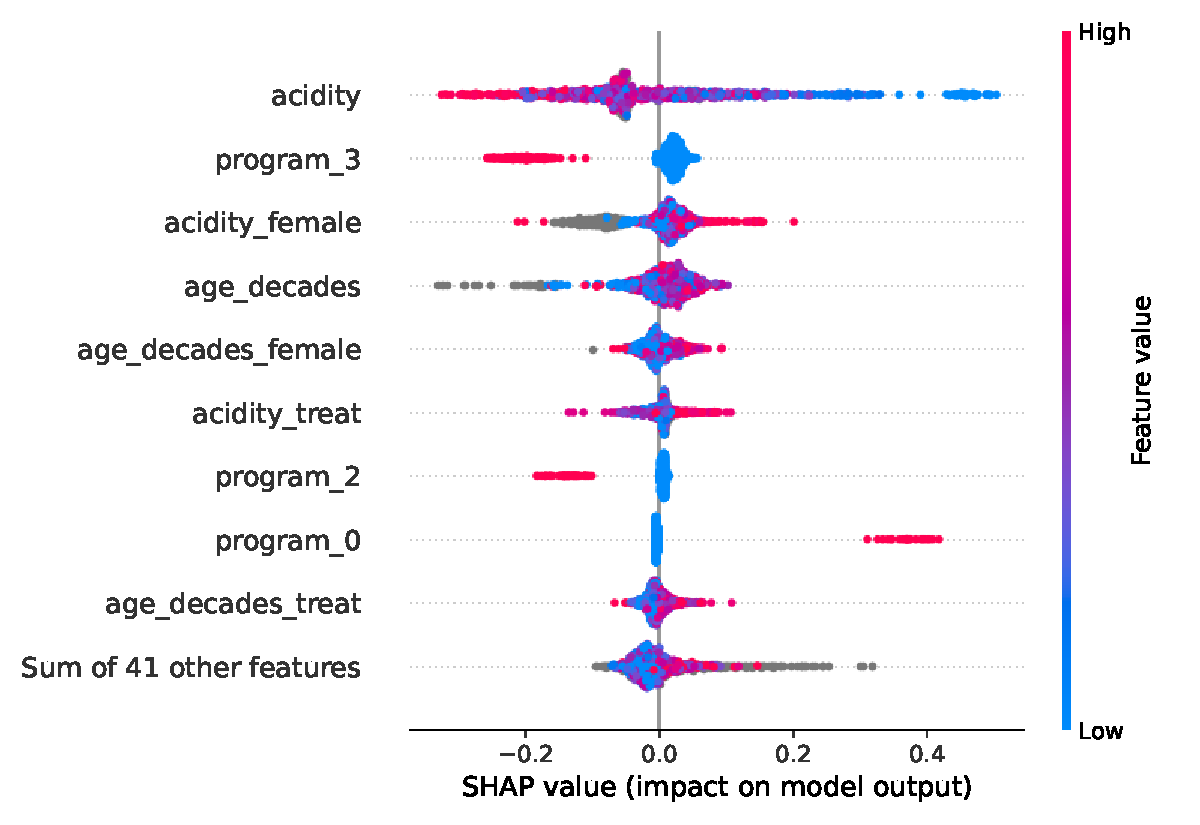
\includegraphics[width=0.7\textwidth]{../output/shap_beeswarm_fert.pdf}
    \begin{minipage}{0.7\textwidth}
    \tiny
    Shapley values estimate how much each feature value contributes to the model's estimated probability of following recommendations for lime/fertilizer. A higher SHAP value (the x-axis) means that the model predicts a higher probability than it would without that feature. Shown here are the top 10 features by average absolute SHAP value. Dots in this graph are blue when the respective feature is a lower value, and red when the respective feature is a higher value. Gray dots indicate missing values for the respective feature.
    \end{minipage}
    \label{fig:shap_fert}
\end{figure}

The distributions of values in Figure \ref{fig:shap_fert} for predicting fertilizer adoption show clear signs of differences between the experiments: 3 of the top 10 variables by average absolute Shapley value are indicators for being in different experiments. Moreover, the chart shows that there are homogenous predicted effects: being in program 3 or program 2 results in a lower predicted adoption rate, while being in program 0 results in a higher predicted adoption rate. Acidity is also important in the model's prediction, though with an unexpected relationship: more acidic soil (lower pH) has a lower predicted adoption rate of fertilizer, while less acidic soil (higher pH) has a higher predicted adoption rate. This could be due to mental fatigue, where farmers with acidic soil feel they can only handle dealing with one problem at a time, in this case dealing with acidic soil by applying lime.

\section{Discussion}
\label{section:discussion}

\subsection{Model Performance}
The fact that AUROC and balanced accuracy both improve when we incorporate additional controls suggests that there is heterogeneity in adopting lime and fertilizer. Further, with AUROC values of 0.84 and 0.86 for lime and fertilizer, respectively, the models are able to predict the adoption of recommended products significantly better than random guessing.\footnote{According to \textcite{mandrekar_receiver_2010}, an AUROC between 0.8 and 0.9 is considered to be excellent at discriminating classes.} While these are non-trivial improvements over the models in \textcite{fabregas_digital_2025}, the original models already provide a fairly high accuracy. To understand whether a more sophisticated machine learning approach is warranted for developing text campaigns, we would need to weigh the costs of additional data collection and modelling against the benefits of more accurate prediction.

Perhaps the most useful implication of our analysis for development economists is the finding that some types of people are more receptive to text message nudges than others, and that these people can be identified with a well-specified model. However, additional research is needed to understand not just the subpopulations that should be targeted for more effective campaigns, but to identify which type of text message works best for each person. As discussed above, text messages are cheap to send, and so developing countries should aim to send messages to all farmers with a mobile phone. Our argument, which we explore below, is that sophisticated models should be developed to automatically cater the message content to the individual farmer so that they maximize the probability of adopting profitable technologies. To develop these models, further work is needed to explore how the properties of a given text message interact with the characteristics of the farmer to influence their probability of adoption.

\subsection{Limitations}

As discussed above, while \textcite{fabregas_digital_2025} greatly improved the data sample size over existing work, a key limitation of their data is that the control variables are not consistent across the various studies. Although LightGBM models can handle missing values in the control variables, the models lose out on statistical precision (and can be biased in some cases) compared to complete data collection. In order to properly harness the power of machine learning and other statistical techniques, further experiments should develop a comprehensive suite of farmer demographics to better identify treatment heterogeneity. If possible, cross-referencing the farmers against a government census could provide a rich set of additional information for modeling the probability of adoption. To the extent that non-governmental organizations (NGOs) or the World Bank Group have already collected such data, it should be used in future experiments. Further, to the extent that local governments have an existing directory of mobile phone numbers for farmers, this could be used to reduce the selection bias of farmers agreeing to sign up for an experiment.

Perhaps the key limitation of text experiments overall is that they require mobile phones. As we showed above, mobile phone ownership has increased dramatically, even in developing countries. But the fact that the poorest people are least likely to own a phone means that a significant proportion of farmers in developing countries likely still do not own a phone. Hopefully, continued development policies and improvements in technology should increase phone ownership in the poorest areas of the world, making text experiments more effective over time.

\subsection{Policy Implications}

\textcite{fabregas_digital_2025} find that text messages can be effective in convincing poor farmers to adopt profit-increasing technology. We show that the adoption rate varies by farmer demographics. Future work should more closely study the factors that maximize a farmer's receptiveness not just to text messages overall, but in identifying the specific types of messages that the farmer will identify with. \textcite{aker_promise_2016} explain that sociocultural factors affect the adoption of technology, and so text-based development programs would benefit from catering the texts to the individual. Below, we discuss some ideas for how text programs could embrace heterogeneity.

The recent advent of generative artificial intelligence (AI) opens up several opportunities for improving text-based development programs. Newly-trained AI models are fluent in many languages, with a new model created by ETH Zurich reported to have fluency in over 1000 languages.\footnote{\url{https://ethz.ch/en/news-and-events/eth-news/news/2025/07/a-language-model-built-for-the-public-good.html}. The model is expected to be released during the summer of 2025.} Such models can improve text programs by translating the information into the farmer's spoken language, as opposed to sending the texts only in English. Additionally, a sophisticated model would know the local dialect and familiar terms that would be most receptive to farmers in a particular geography. Using AI would allow governments to scale text programs to the entire nation without the expensive cost of translation, which is particularly important in African countries with many spoken languages.\footnote{For example, Uganda reportedly has 41 spoken languages today. \url{https://www.ruhr-uni-bochum.de/engling/research/uganda/index.html.en}.}

A key driver for text program success is in reducing the complexity of the message while retaining important information. As we reported above, low literacy rates are a bottleneck in Kenya and Uganda, but text messages need not necessarily require literacy. A carefully crafted series of emojis, pictures, and videos could convey helpful information without requiring text comprehension. Since one of the benefits of text programs is timely salience (as in \textcite{carrion-yaguana_promoting_2020}), it could be that a simple infographic reminding the farmer of lime, fertilizer, or other best practices would improve adoption rates.

To identify the text messages that maximize probability of adopting best practices, researchers need to study a diverse range of text messages simultaneously. AI could be of assistance here as well, providing the ability to rapidly develop new messages with a wide range of emotional content, information detail, language complexity, and other factors, with comparatively little manual input from researchers.

While it would be more expensive than a static message program, the next few years could see the development of an interactive messaging platform in which farmers engage with an AI assistant to obtain personalized informative content. Allowing farmers to interact with the text platform could improve participation and provide a stream of new data to further improve the text suggestions. AI platforms could learn from a user's previous messages to provide highly-individualized responses to maximize their profitability. 

\section{Conclusion}
\label{section:conclusion}

Economic development policies often focus on large-scale structural changes to improve institutions, but an equally powerful avenue for development is improving the economic decisions of the individual. Behavioral economics helps us to understand why farmers fail to adopt profitable technology, and how timely reminders can nudge them towards making better decisions. With the now-widespread adoption of mobile phones in developing countries, text messaging has become an important delivery mechanism for experiments. Such experiments have had somewhat mixed results, but \textcite{fabregas_digital_2025} show that they can significantly improve the adoption of lime and fertilizer among poor famers in Kenya and Uganda. We additionally show that there is significant heterogeneity in responsiveness to text programs, in spite of data availability issues. Looking forward, text programs should embrace this heterogeneity with the aim of creating personalized messages that maximize farmers' adoption of profitable technologies. These small improvements, implemented at a national scale, could be a highly cost-efficient policy acting in tandem with existing programs.

\newpage
\printbibliography
\newpage

\section{Appendix}

\subsection{Receiver Operating Curves}
\begin{figure}[H]
    \centering
    \caption{Receiver Operating Curve, Large Model: Lime}
    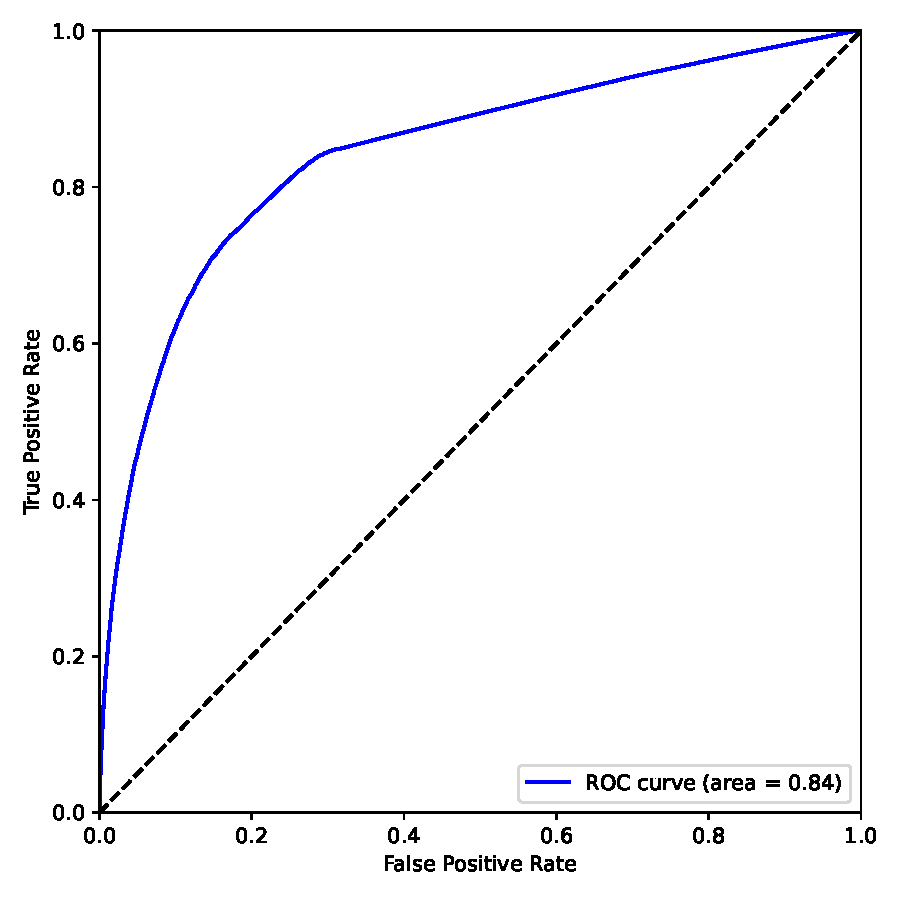
\includegraphics[width=0.5\textwidth]{../output/lightgbm_roc_lime.pdf}
    \begin{minipage}{0.6\textwidth}
    \tiny
    The receiver operating characteristic (ROC) curve depicts the performance of a binary classification model across varying decision thresholds. The curve illustrates the trade-off between true positive rate and false positive rate, and the area under the ROC curve (AUROC) quantifies the model's overall ability to discriminate between the two outcome classes. According to \textcite{mandrekar_receiver_2010}, an AUROC between 0.8 and 0.9 is considered to be excellent at discriminating classes.
    \end{minipage}
    \label{fig:roc_lime}
\end{figure}

\begin{figure}[H]
    \centering
    \caption{Receiver Operating Curve, Large Model: Fertilizer}
    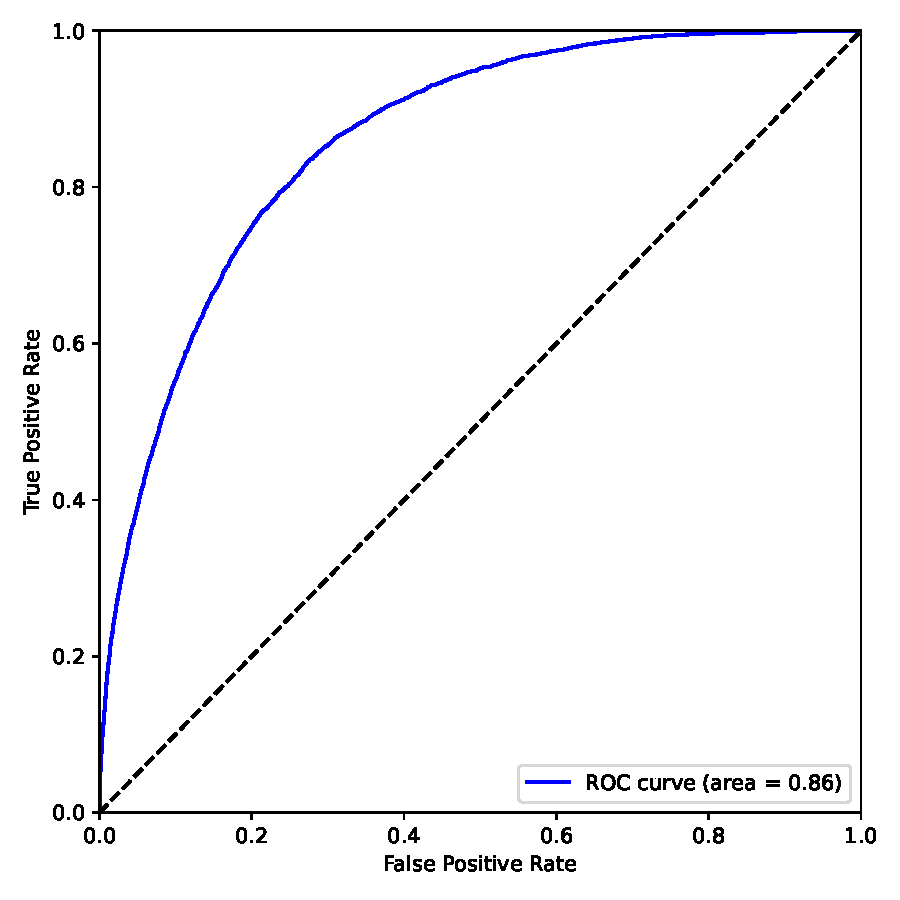
\includegraphics[width=0.5\textwidth]{../output/lightgbm_roc_fert.pdf}
    \begin{minipage}{0.6\textwidth}
    \tiny
    The receiver operating characteristic (ROC) curve depicts the performance of a binary classification model across varying decision thresholds. The curve illustrates the trade-off between true positive rate and false positive rate, and the area under the ROC curve (AUROC) quantifies the model's overall ability to discriminate between the two outcome classes. According to \textcite{mandrekar_receiver_2010}, an AUROC between 0.8 and 0.9 is considered to be excellent at discriminating classes.
    \end{minipage}
    \label{fig:roc_fert}
\end{figure}

\subsection{Combined Model}
\label{sec:combined_model}
The combined model was created by stacking the datasets for lime and fertilizer adoption. Note that creating the dataset this way duplicates records for some farmers who were asked to consider buying both lime and fertilizer. The combined dataset has 170,021 observations.

\begin{figure}[H]
    \centering
    \caption{Receiver Operating Curve, Large Model: Lime/Fertilizer}
    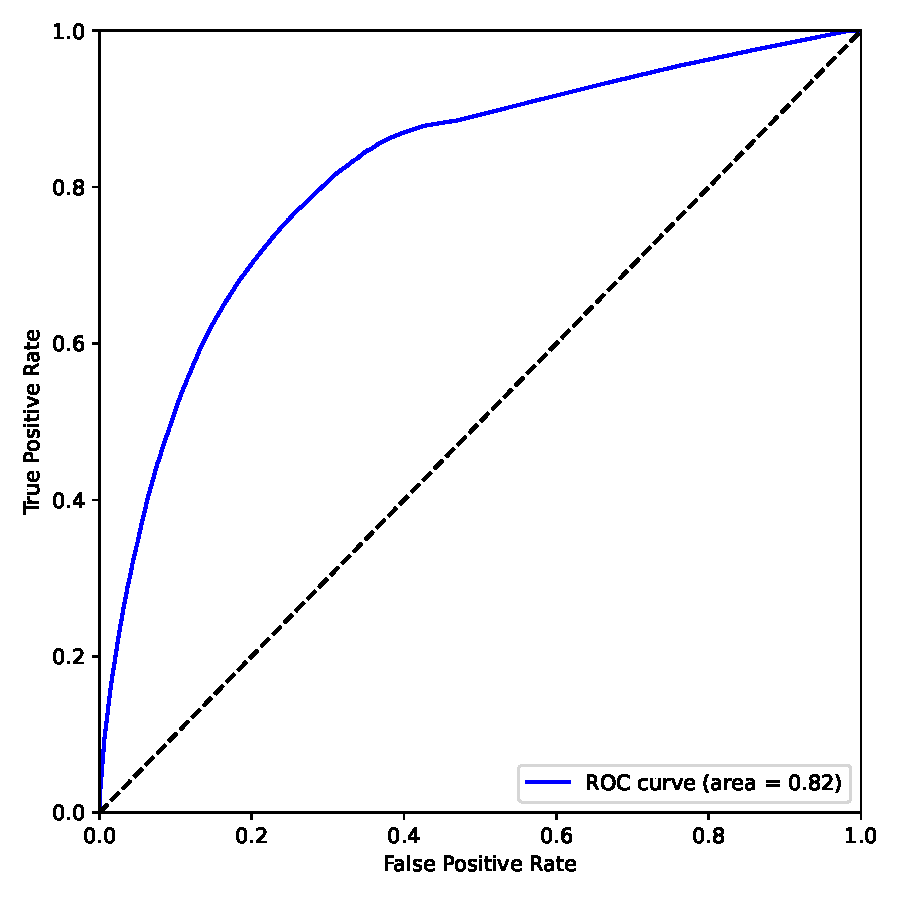
\includegraphics[width=0.5\textwidth]{../output/lightgbm_roc_combined.pdf}
    \begin{minipage}{0.6\textwidth}
    \tiny
    The receiver operating characteristic (ROC) curve depicts the performance of a binary classification model across varying decision thresholds. The curve illustrates the trade-off between true positive rate and false positive rate, and the area under the ROC curve (AUROC) quantifies the model's overall ability to discriminate between the two outcome classes. According to \textcite{mandrekar_receiver_2010}, an AUROC between 0.8 and 0.9 is considered to be excellent at discriminating classes.
    \end{minipage}
    \label{fig:roc_combined}
\end{figure}

\begin{figure}[H]
    \centering
    \caption{Top Shapley Value Distributions, Large Model: Lime/Fertilizer}
    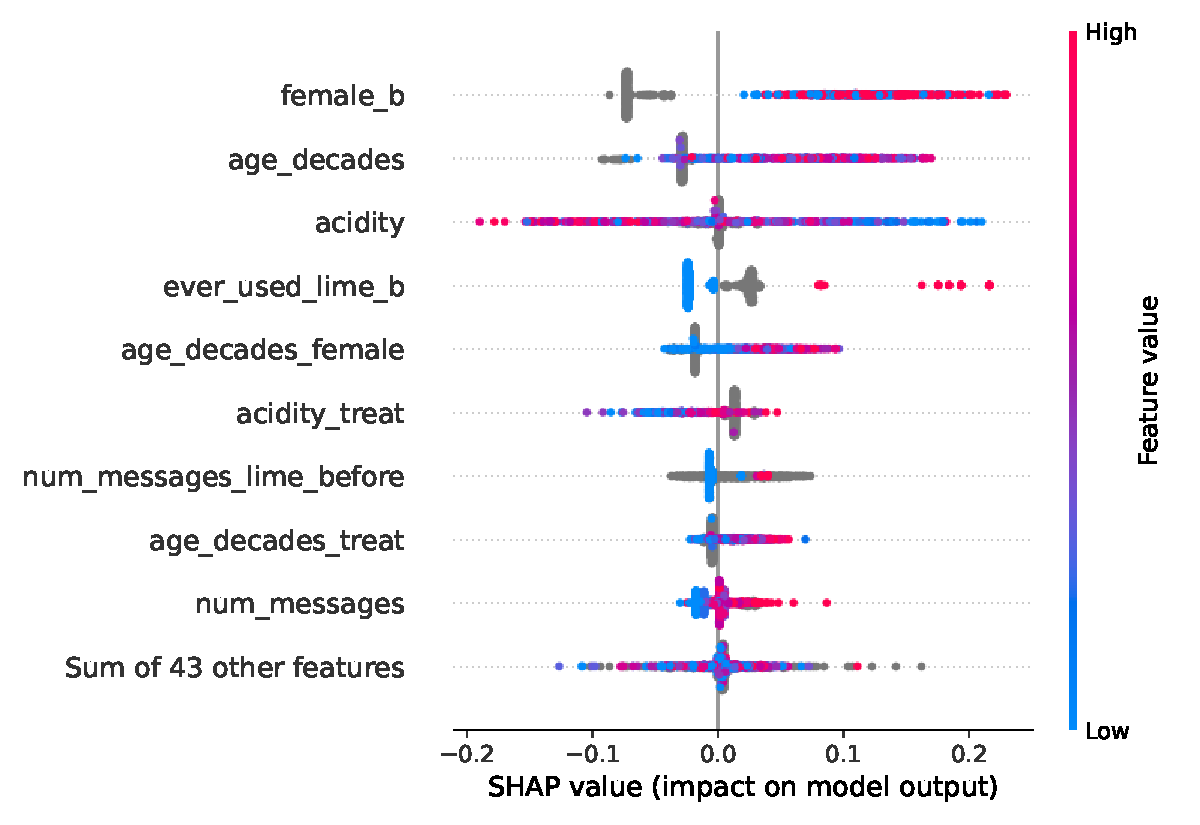
\includegraphics[width=0.7\textwidth]{../output/shap_beeswarm_combined.pdf}
    \begin{minipage}{0.7\textwidth}
    \tiny
    Shapley values estimate how much each feature value contributes to the model's estimated probability of following recommendations for lime/fertilizer. A higher SHAP value (the x-axis) means that the model predicts a higher probability than it would without that feature. Shown here are the top 10 features by average absolute SHAP value. Dots in this graph are blue when the respective feature is a lower value, and red when the respective feature is a higher value. Gray dots indicate missing values for the respective feature.
    \end{minipage}
    \label{fig:shap_combined}
\end{figure}

\end{document}